\section{Limitaciones Técnicas y Desafíos}
A pesar de los avances sobresalientes documentados en la literatura científica reciente, los autores de la literatura revisada identifican varios inconvenientes técnicos y operativos recurrentes que restringen la generalización de estas tecnologías en la práctica \cite{huang2025dtldetector, alshehri2025integrated, xie2025yoloace}.

\subsection{Variabilidad Lumínica y Oclusión}
Los cambios repentinos en las condiciones de iluminación, tales como la transición rápida al entrar o salir de túneles viales, el deslumbramiento solar directo, las sombras complejas proyectadas por árboles u otras estructuras urbanas, y la conducción puramente nocturna, degradan de forma severa el contraste de las imágenes capturadas \cite{mota2025integration, kavitha2025towards}. Esto incrementa sustancialmente los falsos negativos en modelos de detección facial o de seguimiento vehicular \cite{salakapuri2025integrated, rachoti2025traffic}. 

Adicionalmente, la oclusión parcial o total de objetos (por ejemplo, camiones de gran tonelaje bloqueando la línea de visión de cámaras fijas respecto a peatones o vehículos pequeños en cruces) continúa siendo un problema técnico complejo \cite{elhenidy2025gyyolo, mota2025integration}. En el monitoreo de conductores, las oclusiones debidas al uso de anteojos de sol, tapabocas o movimientos naturales de las manos sobre el volante representan fuentes críticas de error que interrumpen el rastreo de marcas faciales esenciales \cite{silva2025light, deshpande2025computervision}.

\subsection{Restricciones de Hardware y Requerimientos de Tiempo Real}
El procesamiento a alta velocidad (típicamente a más de 30 FPS) es una condición indispensable para garantizar la seguridad activa y alertar a tiempo al conductor o al centro de monitoreo de tráfico. Sin embargo, los modelos de Deep Learning más precisos conllevan una alta complejidad paramétrica y un elevado consumo energético, lo que limita su despliegue en hardware de bajo costo y potencia reducida (Edge Computing) \cite{komol2024prediction, hernandez2024realtime}. Esto fuerza la necesidad de aplicar técnicas avanzadas de optimización, tales como la cuantización de modelos a precisión de 8 bits, la destilación de conocimiento (knowledge distillation) de redes grandes a redes pequeñas y la poda de canales (channel pruning) \cite{abdullah2025lcyolo, bhaskara2025deep}, asumiendo en ocasiones una pérdida marginal en la exactitud a cambio de viabilidad operativa.

Aunado a la latencia intrínseca de los modelos, la sincronización temporal y espacial de múltiples flujos de video en tiempo real representa otro desafío operativo de gran envergadura en despliegues prácticos \cite{suresh2025traffic, owais2025light}. En entornos urbanos donde se recopila información de múltiples cámaras de CCTV en intersecciones contiguas, o en sistemas a bordo que integran sensores ópticos periféricos para cubrir los puntos ciegos del vehículo, la falta de alineación de tiempo en milisegundos (jitter de red) puede provocar falsas detecciones de velocidad o errores en el seguimiento continuo (multi-camera tracking) de un mismo vehículo a través de la red vial. Esta desalineación temporal deteriora la precisión de la reconstrucción tridimensional de la escena y limita la confiabilidad del sistema ante eventos dinámicos rápidos.

\subsection{Sesgo en los Datos y Generalización}
Una limitación crítica compartida por gran parte de los estudios analizados es el desequilibrio en los conjuntos de datos de entrenamiento \cite{alshehri2025integrated, lu2024validation}. La mayoría de los datasets públicos de fatiga y distracción se graban bajo entornos de laboratorio controlados con un número limitado de sujetos y condiciones de luz uniformes \cite{wu2025visual, usman2024distracted}. Al transferir estos modelos preentrenados a escenarios del mundo real, se observa una degradación drástica del rendimiento, lo que resalta la falta de capacidad de generalización entre dominios cruzados (cross-domain generalization) \cite{mulhall2023european, galloway2023evaluation}. Asimismo, existe un sesgo demográfico marcado en los conjuntos de datos de rostros, lo que afecta la exactitud de los algoritmos de detección en personas con distintos rasgos étnicos o estructuras faciales no representadas en los datos de entrenamiento iniciales.

La Fig.~\ref{fig:cruce_limitaciones} muestra la distribución cruzada de la incidencia de estas limitaciones según el enfoque metodológico de los artículos científicos analizados.

\begin{figure}[htbp]
\centerline{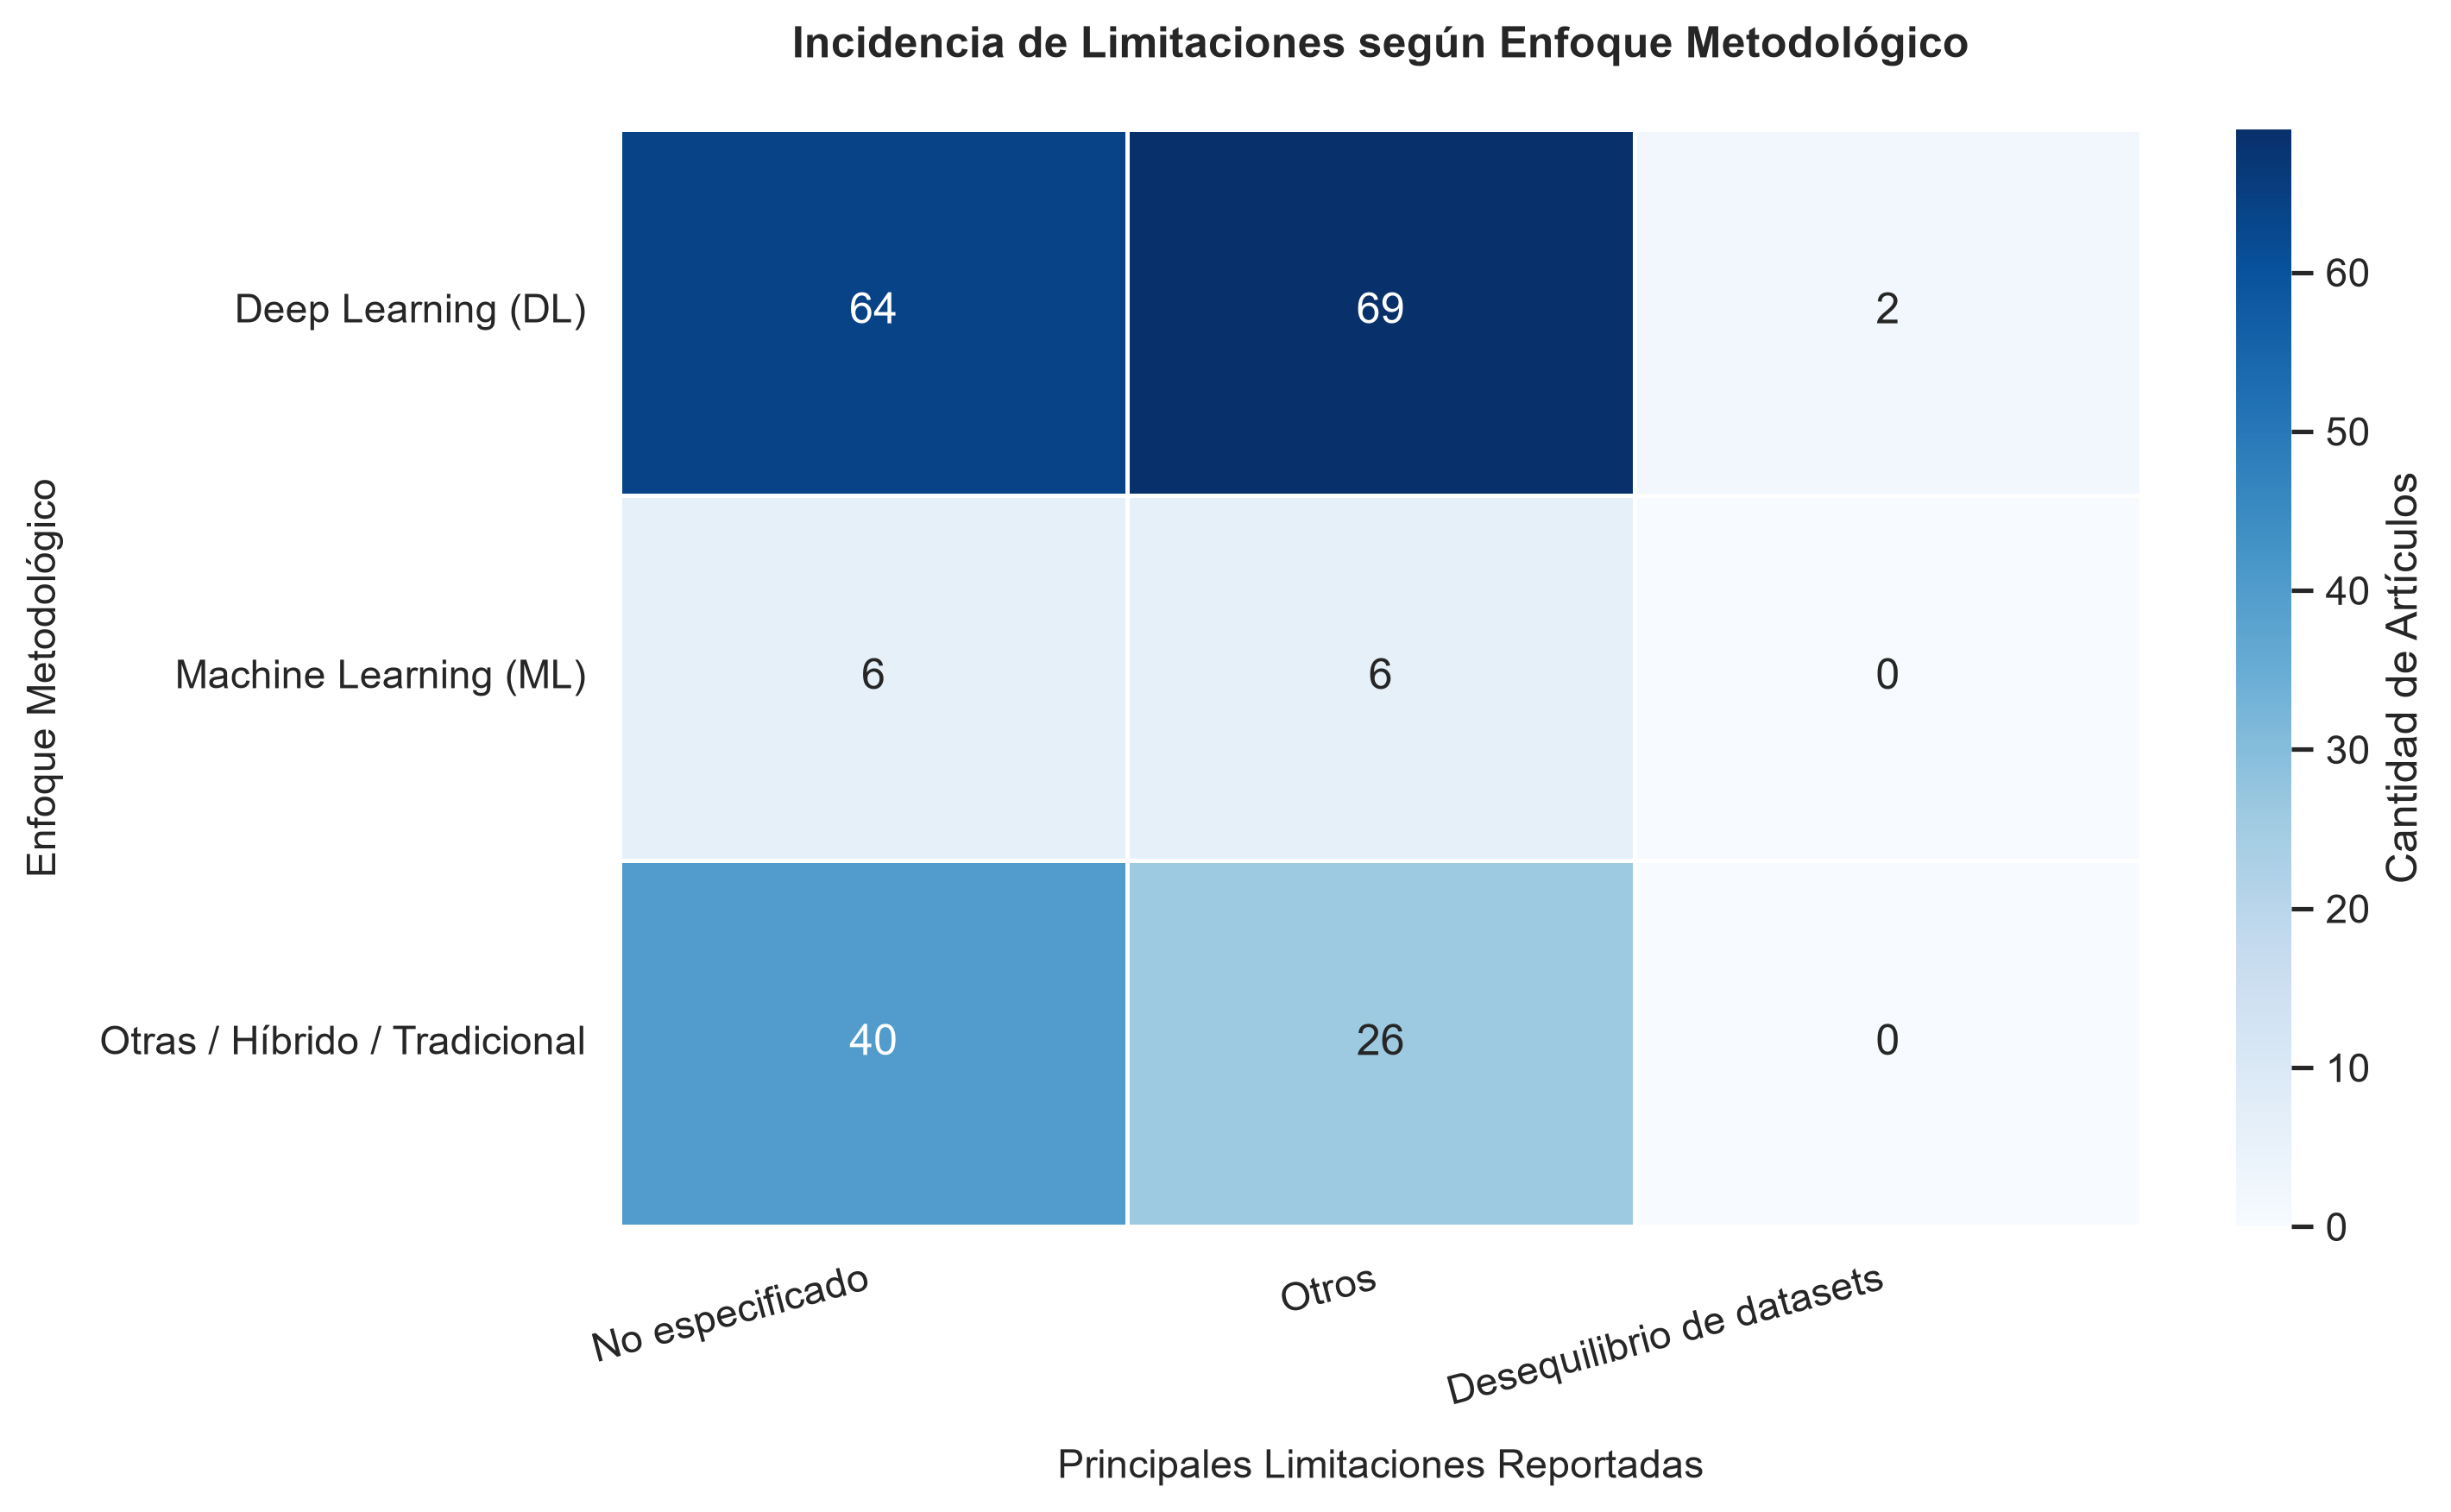
\includegraphics[width=0.48\textwidth]{../graficos/19_cruce_limitaciones_metodologia.png}}
\caption{Incidencia de Limitaciones según el Enfoque Metodológico de la Investigación.}
\label{fig:cruce_limitaciones}
\end{figure}

Para complementar esta perspectiva, la Fig.~\ref{fig:cruce_limitaciones_entorno} correlaciona la presencia de estos desafíos técnicos frente a los entornos de validación experimental. Se evidencia que los problemas de iluminación y la oclusión visual predominan en cámaras de circuito cerrado (CCTV) debido a factores climáticos descontrolados \cite{rachoti2025traffic, kumar2025smart}, mientras que la latencia y restricciones de hardware crítico representan los mayores obstáculos en el despliegue embebido a bordo y en vehículos aéreos (UAV) \cite{poudel2024improved, bakirci2024enhancing}.

\begin{figure}[htbp]
\centerline{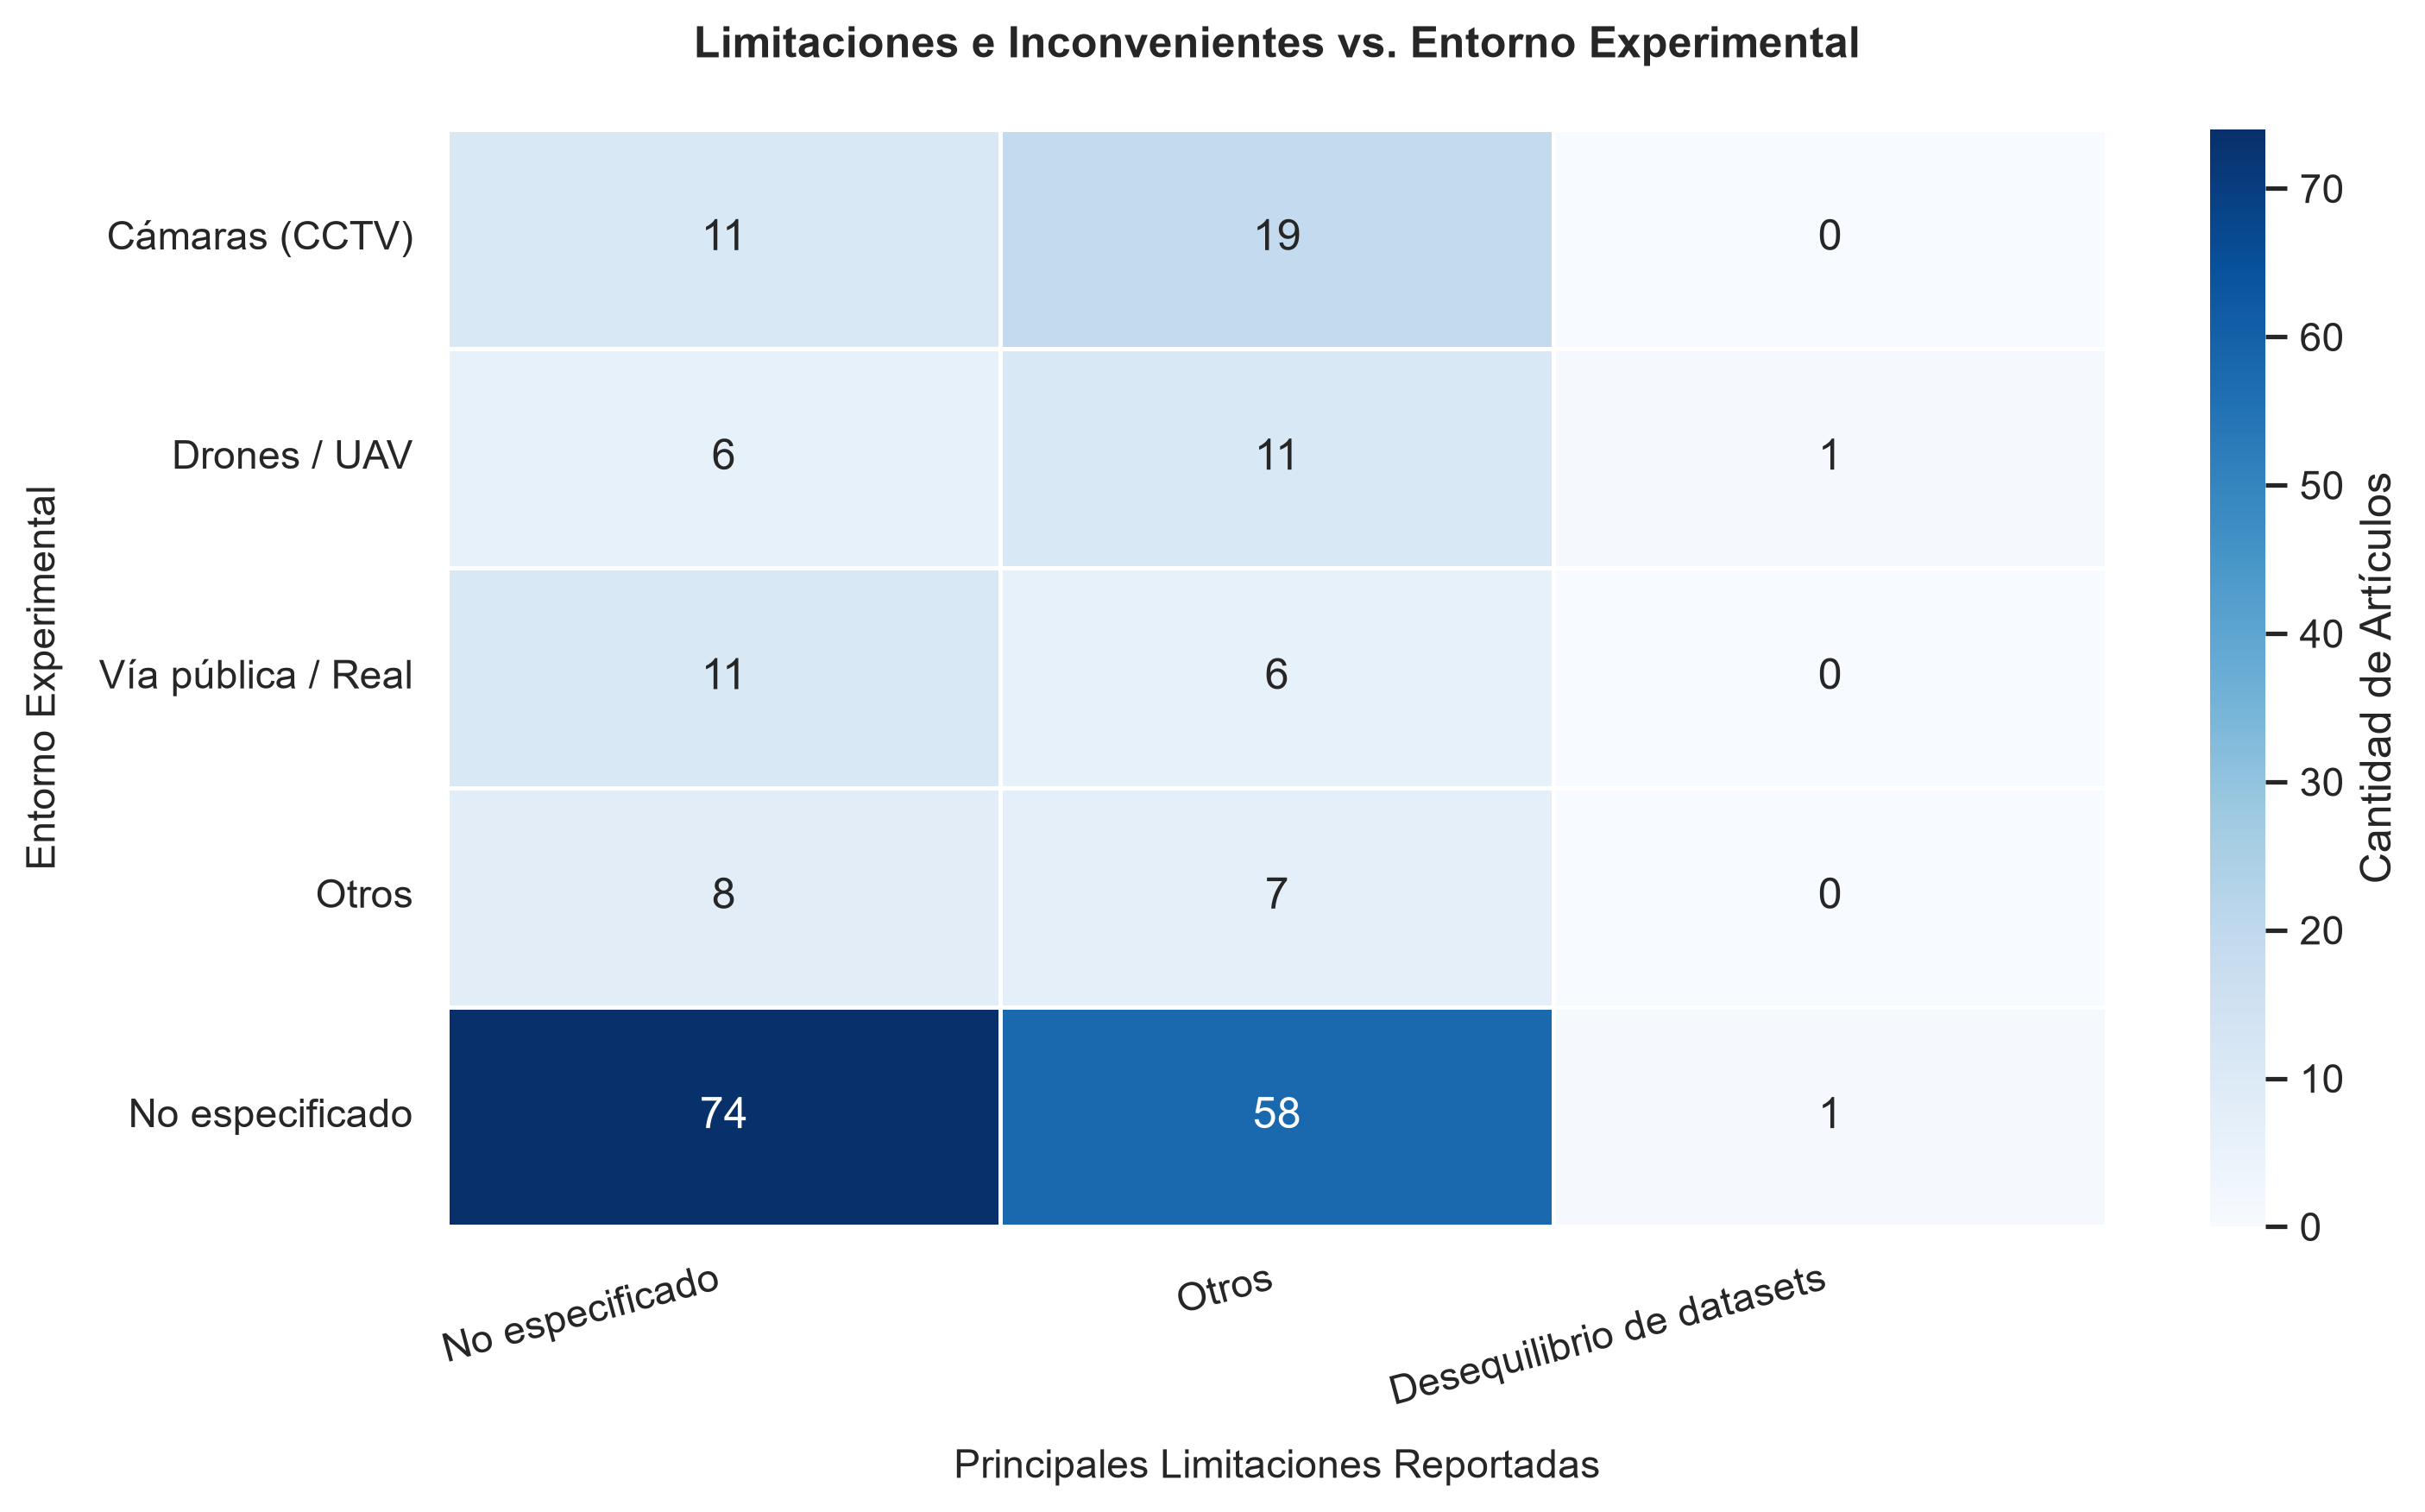
\includegraphics[width=0.48\textwidth]{../graficos/22_cruce_limitaciones_entorno.png}}
\caption{Correlación de Limitaciones e Inconvenientes vs. Entorno Experimental.}
\label{fig:cruce_limitaciones_entorno}
\end{figure}

\subsection{Desafíos de Privacidad, Ética y Seguridad de Datos}
El despliegue masivo de sistemas de monitoreo de conductores y cámaras de videovigilancia urbana plantea serios desafíos éticos y de privacidad de datos que deben ser abordados rigurosamente por los diseñadores de políticas públicas y desarrolladores de tecnología \cite{gowroju2025urbaneye, pujitha2025traffic}. La captura continua del rostro del conductor, el análisis de sus expresiones emocionales y el seguimiento de su mirada recopilan información biométrica de carácter altamente sensible. Si estos datos son transmitidos sin encriptación o almacenados de manera centralizada en servidores de la nube, se crea un riesgo latente de vulneración de la privacidad y acceso no autorizado por terceros \cite{balasaranya2025realtime, uddin2025abnormal}.

Normativas internacionales estrictas, como el Reglamento General de Protección de Datos (GDPR) en Europa, exigen que el procesamiento de datos biométricos se realice bajo principios de minimización de datos y consentimiento explícito. In respuesta a estos desafíos, la tendencia actual en el estado del arte se orienta fuertemente hacia el procesamiento en el borde (Edge Computing), donde la inferencia del modelo se ejecuta directamente dentro del hardware instalado en el vehículo (por ejemplo, microcontroladores avanzados o procesadores embebidos NVIDIA Jetson) \cite{nell2025classification, sorum2025modeling}. Al procesar las imágenes localmente y descartar de inmediato los fotogramas del video, transmitiendo únicamente alertas de metadatos (como "somnolencia detectada"), se resguarda de forma efectiva la identidad y privacidad del conductor, garantizando al mismo tiempo una baja latencia en la emisión de advertencias de seguridad.

Para mitigar los riesgos asociados con la transmisión de videos biométricos sensibles a servidores en la nube, el Aprendizaje Federado (Federated Learning) se posiciona como una solución altamente prometedora en la literatura reciente \cite{ijaradar2025datadriven, wang2025application}. Bajo este paradigma, los dispositivos embebidos en el borde a bordo de múltiples vehículos entrenan de forma colaborativa un modelo global compartiendo únicamente las actualizaciones de gradientes cifrados, sin exponer jamás la información biométrica cruda o el video del rostro a servidores centrales. Esto no solo garantiza el cumplimiento de normativas de privacidad rigurosas como la GDPR \cite{kumar2025smart, kalwa2025unusual}, sino que también reduce sustancialmente el ancho de banda necesario en redes móviles vehiculares (V2X).
